%% This is the ctufit-thesis example file. It is used to produce theses
%% for submission to Czech Technical University, Faculty of Information Technology.
%%
%% This is version 1.3.10, built 27. 2. 2025.
%% 
%% Get the newest version from
%% https://gitlab.fit.cvut.cz/theses-templates/FITthesis-LaTeX
%%
%%
%% Copyright 2024, Tomas Novacek
%% Copyright 2021, Eliska Sestakova and Ondrej Guth
%%
%% This work may be distributed and/or modified under the
%% conditions of the LaTeX Project Public License, either version 1.3
%% of this license or (at your option) any later version.
%% The latest version of this license is in
%%  https://www.latex-project.org/lppl.txt
%% and version 1.3 or later is part of all distributions of LaTeX
%% version 2005/12/01 or later.
%%
%% This work has the LPPL maintenance status `maintained'.
%%
%% The current maintainer of this work is Tomas Novacek.
%% Alternatively, submit bug reports to the tracker at
%% https://gitlab.fit.cvut.cz/theses-templates/FITthesis-LaTeX/issues
%%
%%

% arara: xelatex
% arara: biber
% arara: xelatex
% arara: xelatex

%%%%%%%%%%%%%%%%%%%%%%%%%%%%%%%%%%%%%%%%%
% CLASS OPTIONS
% language: czech/english/slovak
% thesis type: bachelor/master/dissertation
% colour: bw for black&white OR no option for default colour scheme
% electronic (oneside) or printed (twoside), twoside is default
% paragraph - if passed, this optional argument sets paragraphs as the deepest level of headers, styles it, numbers it and adds it to Table of Content. Use with care! Normally, it is considered unwise to use it, since its too deep.
%%%%%%%%%%%%%%%%%%%%%%%%%%%%%%%%%%%%%%%%%
\documentclass[english,bachelor,unicode,oneside]{ctufit-thesis}

% helper package for todo notes
\usepackage[color=green,  textsize=scriptsize, loadshadowlibrary]{todonotes}

% set the default options for all \todo calls
\setuptodonotes{
  color=gray!30,
  shadow}



% custom styles for high, medium and low priorities
\todostyle{h}{color=red!30, shadow}
\todostyle{m}{color=yellow!30, shadow}
\todostyle{l}{color=blue!30, shadow}


\usepackage{import}

\usepackage[hybrid]{markdown}

\usepackage{environ}

% To turn off markdown completely use this command
% it will make markdow blocks as normal ones
% \RenewEnviron{markdown}{\BODY}

\usepackage{booktabs}

\usepackage{subcaption}

% package to prevent figures overfloating to other sections
\usepackage{placeins}

\usepackage{listings}
\usepackage{xcolor}
\usepackage{minted}

% for the medium
\usepackage{dirtree}

\input{utils/custom_commands}


%%%%%%%%%%%%%%%%%%%%%%%%%%%%%%%%%%
% FILL IN THIS INFORMATION
%%%%%%%%%%%%%%%%%%%%%%%%%%%%%%%%%%
\ctufittitle{Enhancing Fake News Classification with Advanced NLP Models} % replace with the title of your thesis
\ctufitauthorfull{Nikita Bardatskii} % replace with your full name (first name(s) and then family name(s) / surname(s)) including academic degrees
\ctufitauthorsurnames{Bardatskii} % replace with your surname(s) / family name(s)
\ctufitauthorgivennames{Nikita} % replace with your first name(s) / given name(s)
\ctufitsupervisor{doc.\,Ing.\,Ladislava Smítková Janků,\,Ph.D.} % replace with name of your supervisor/advisor (include academic degrees)
\ctufitdepartment{Department of Applied Mathematics} % replace with the department of your defence
\ctufityear{2026} % replace with the year of your defence
\ctufitdeclarationplace{Prague} % replace with the place where you sign the declaration
\ctufitdeclarationdate{\today} % replace with the date of signature of the declaration

% DO NOT REMOVE - breaks everything
\ctufitabstractCZE{Tato studie navazuje na předchozí výzkum, ve kterém byly pro klasifikaci zpravodajských článků nebo jejich shrnutí jako falešných nebo důvěryhodných použity relativně jednoduché klasické modely strojového učení. Cílem této práce je prozkoumat využití pokročilejších architektur — konkrétně modelů založených na transformerech — za účelem zlepšení klasifikační výkonnosti na stejných datových sadách, které byly použity v předchozí studii.}
\ctufitabstractENG{This study extends prior research in which relatively simple, classical machine learning models were employed to classify news articles or summaries as either fake or reliable. The objective of the present work is to investigate the use of more advanced architectures—specifically transformer-based models—to enhance classification performance on the same datasets utilized in the previous study.}
\ctufitkeywordsCZE{transformery, BERT, DistillBERT, RoBERTa, GPT falešné zprávy, hluboké učení, zpracování přirozeného jazyka, binární klasifikace}
\ctufitkeywordsENG{transformers, BERT, DistillBERT, RoBERTa, GPT, fake news, deep learning, natural language processing, binary classification}

%%%%%%%%%%%%%%%%%%%%%%%%%%%%%%%%%%
% END FILL IN
%%%%%%%%%%%%%%%%%%%%%%%%%%%%%%%%%%

%%%%%%%%%%%%%%%%%%%%%%%%%%%%%%%%%%
% CUSTOMIZATION of this template
% Skip this part or alter it if you know what you are doing.
%%%%%%%%%%%%%%%%%%%%%%%%%%%%%%%%%%

\RequirePackage{iftex}[2020/03/06]
\iftutex % XeLaTeX and LuaLaTeX
    \RequirePackage{ellipsis}[2020/05/22] %ellipsis workaround for XeLaTeX
\else
    \errmessage{Onl in Overleaf
y compilation with XeLaTeX or LuaLaTeX is allowed}
    \stop
\fi

% hyperlinks
\hypersetup{
    pdfpagelayout=TwoPageRight,
    colorlinks=false,
    allcolors=decoration,
    pdfborder={0 0 0.1}
}

% uncomment the following to hide all hyperlinks
%\hypersetup{hidelinks}

% uncomment the following to change the colour of all hyperlinks to CTU blue
%\hypersetup{allbordercolors=decoration}

\RequirePackage{pdfpages}[2020/01/28]

%%%%%%%%%%%%%%%%%%%%%%%%%%%%%%%%%%
% CUSTOMIZATION of this template END
%%%%%%%%%%%%%%%%%%%%%%%%%%%%%%%%%%


%%%%%%%%%%%%%%%%%%%%%%
% DEMO CONTENTS SETTINGS
% You may choose to modify this part.
%%%%%%%%%%%%%%%%%%%%%%
\usepackage{dirtree}
\usepackage{lipsum,tikz}
\usepackage[style=iso-numeric]{biblatex}
\addbibresource{utils/bib-database.bib}
\usepackage{xurl}
\usepackage{listings} % typesetting of sources
%\usepackage{minted}
\usepackage{csquotes}

%%%%%%%%%%%%%%%%%%%%%%
% DEMO CONTENTS SETTINGS END
%%%%%%%%%%%%%%%%%%%%%%

\begin{document} 
\frontmatter\frontmatterinit % do not remove these two commands

\thispagestyle{empty}\maketitle\thispagestyle{empty}\cleardoublepage % do not remove these four commands


% !!!!!!!!!!!!!!!!!!!!!!!!! include in final version !!!!!!!!!!!!!!!!!!!!!!!!!
% 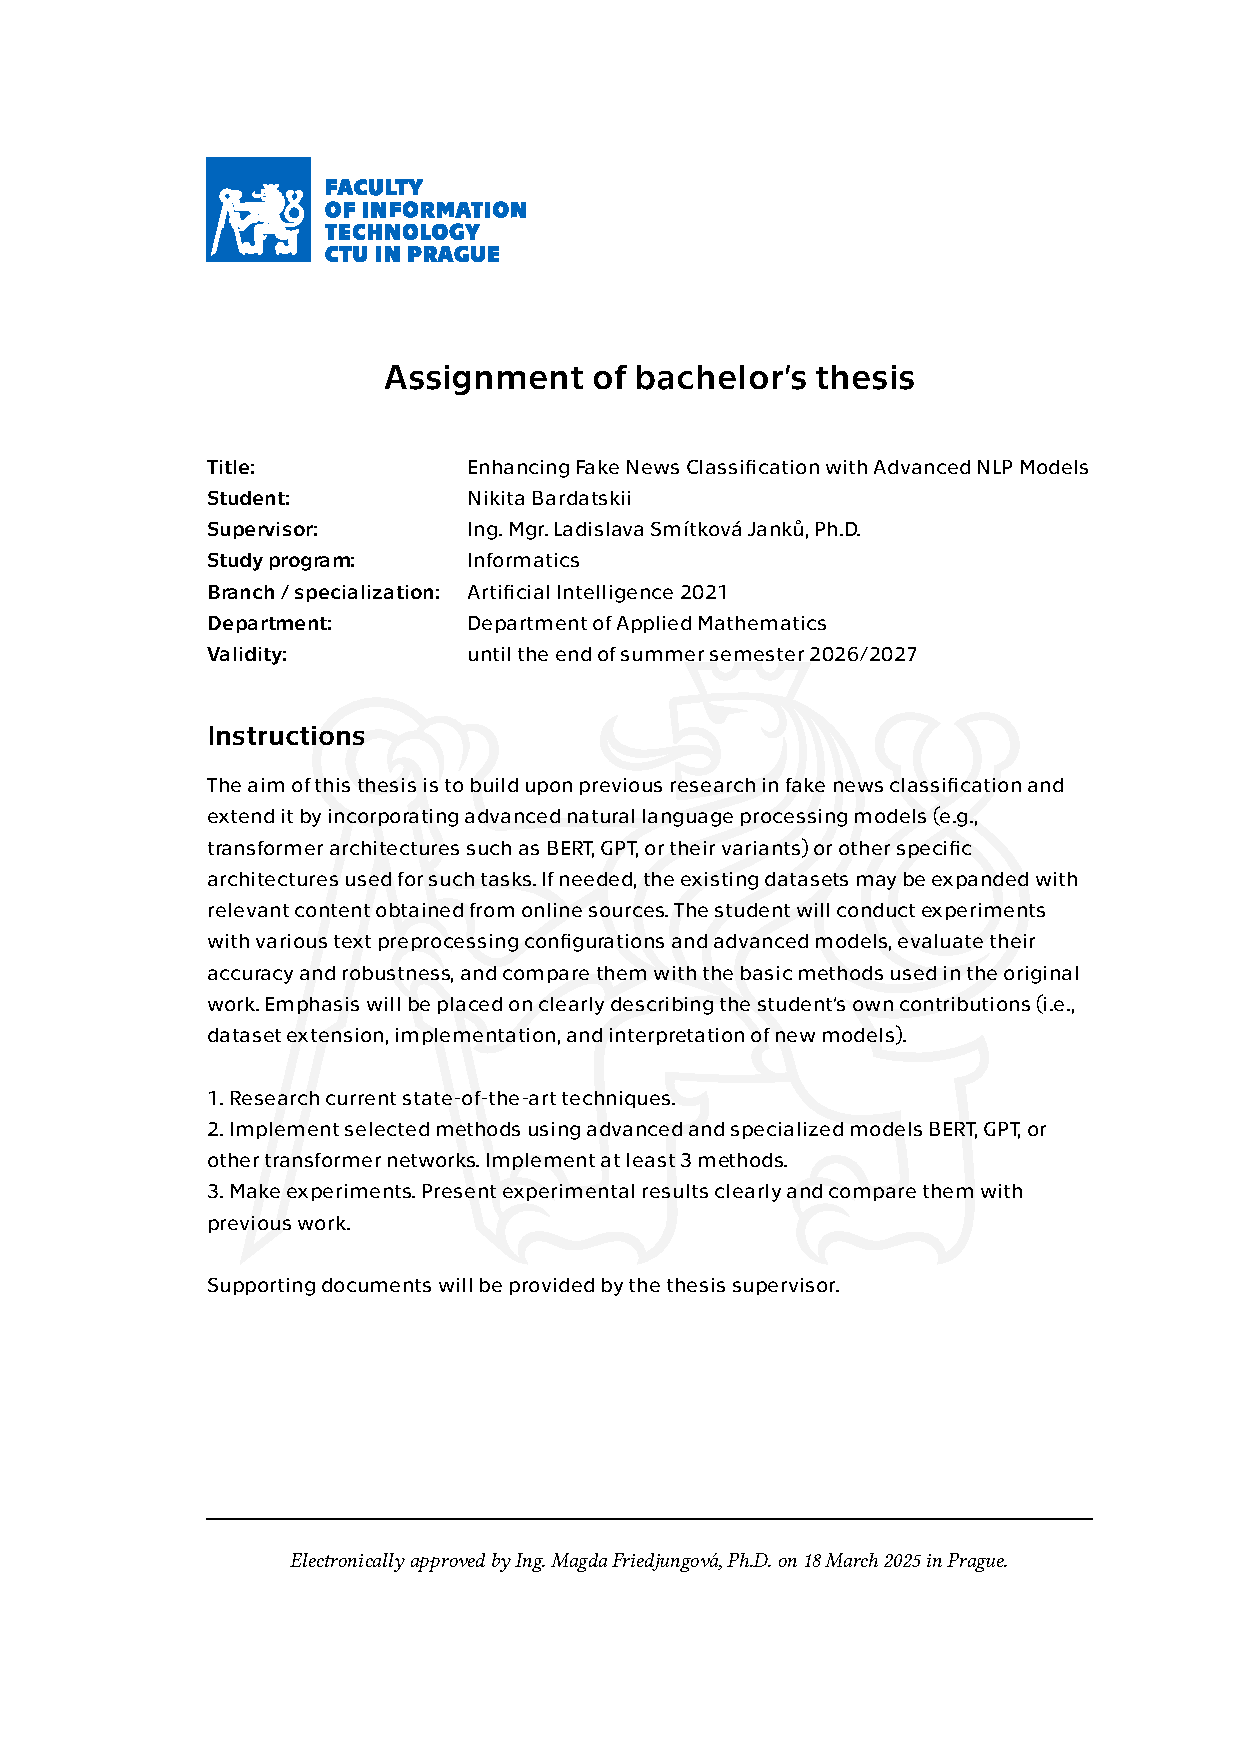
\includepdf[pages={1-}]{text/misc/assignment.pdf} % replace this file with your thesis assignment generated from ProjectsFIT

\imprintpage % do not remove this command
\stopTOCentries
%%%%%%%%%%%%%%%%%%%%%%
% list of other contents END
%%%%%%%%%%%%%%%%%%%%%%
% !!!!!!!!!!!!!!!!!!!!!!!!! include in final version !!!!!!!!!!!!!!!!!!!!!!!!!

%%%%%%%%%%%%%%%%%%%
% ACKNOWLEDGMENT
% FILL IN / MODIFY
% This is a place to thank people for helping you. It is common to thank your supervisor.
%%%%%%%%%%%%%%%%%%%
\begin{acknowledgmentpage}

I would like to express my gratitude to my supervisor, Ing. Mgr. Ladislava Smítková Janků, Ph.D., for providing me with constructive feedback throughout the writing of this thesis. Furthermore, I would like to extend my thanks to the faculty and staff of CTU in Prague for providing a rich learning environment. Finally, I would like to thank my family and friends for their endless patience and support, particularly to my mother and brother for their emotional support, and to my friend Daniel Dajbov, who supported me during the final days of writing this thesis..


\end{acknowledgmentpage} 
%%%%%%%%%%%%%%%%%%%
% ACKNOWLEDGMENT END
%%%%%%%%%%%%%%%%%%%   
% !!!!!!!!!!!!!!!!!!!!!!!!! include in final version !!!!!!!!!!!!!!!!!!!!!!!!!

%%%%%%%%%%%%%%%%%%%
% DECLARATION
% FILL IN / MODIFY
%%%%%%%%%%%%%%%%%%%
% INSTRUCTIONS
% ENG: choose one of approved texts of the declaration. DO NOT CREATE YOUR OWN. Find the approved texts at https://courses.fit.cvut.cz/SFE/download/index.html#_documents (document Declaration for FT in English)
% CZE/SLO: Vyberte jedno z fakultou schvalenych prohlaseni. NEVKLADEJTE VLASTNI TEXT. Schvalena prohlaseni najdete zde: https://courses.fit.cvut.cz/SZZ/dokumenty/index.html#_dokumenty (prohlášení do ZP)
\begin{declarationpage}
\begin{markdown}
I hereby declare that the presented thesis is my own work and that I have cited all sources of
information in accordance with the Guideline for adhering to ethical principles when elaborating an
academic final thesis.

I acknowledge that my thesis is subject to the rights and obligations stipulated by the Act No.
121/2000 Coll., the Copyright Act, as amended, in particular the fact that the Czech Technical
University in Prague has the right to conclude a licence agreement on the utilization of this thesis as
a school work pursuant of Section 60 (1) of the Act.

I declare that I have used AI tools during the preparation and writing of my thesis. I have verified
the generated content. I confirm that I am aware that I am fully responsible for the content of the
thesis. The AI tools were used for the following purposes:
- searching for relevant studies and scientific papers,
- retrieving relevant information from referenced sources,
- improving the readability and coherence of the text.
\end{markdown}
\end{declarationpage}
%%%%%%%%%%%%%%%%%%%
% DECLARATION END
%%%%%%%%%%%%%%%%%%%

\printabstractpage % do not remove this command

%%%%%%%%%%%%%%%%%%%
% SUMMARY
% FILL IN / MODIFY
% OR REMOVE ENTIRELY (upon agreement with your supervisor)
% (appropriate to remove in most theses)
%%%%%%%%%%%%%%%%%%%
% \begin{summarypage}
% \section*{Summary section}
% 
% \lipsum[1][1-8]
% 
% \section*{Summary section}
% 
% \lipsum[2][1-6]
% 
% \section*{Summary section}
% 
% \lipsum[3]
% 
% \section*{Summary section}
% 
% \lipsum[2]
% 
% \section*{Summary section}
% 
% \lipsum[1][1-8] Lorem lorem lorem.
% \end{summarypage}
%%%%%%%%%%%%%%%%%%%
% SUMMARY END
%%%%%%%%%%%%%%%%%%%

\tableofcontents % do not remove this command
%%%%%%%%%%%%%%%%%%%%%%
% list of other contents: figures, tables, code listings, algorithms, etc.
% add/remove commands accordingly
%%%%%%%%%%%%%%%%%%%%%%
\listoffigures % list of figures
\begingroup
\let\clearpage\relax
\listoftables % list of tables
\thectufitlistingscommand
\endgroup

%%%%%%%%%%%%%%%%%%%
% ABBREVIATIONS
%%%%%%%%%%%%%%%%%%%

% DO NOT REMOVE - it breaks numeration of chapters, etc.
%%%%%%%%%%%%%%%%%%%
% ABBREVIATIONS
% FILL IN / MODIFY
% OR REMOVE ENTIRELY
% List the abbreviations in lexicography order.
%%%%%%%%%%%%%%%%%%%
\chapter{\thectufitabbreviationlabel}


\begin{tabular}{rl}
BERT & Bidirectional Encoder Representations from Transformers \\
DistilBERT & Distilled BERT \\
RoBERTa & A Robustly Optimized BERT Pretraining Approach \\
GPT & Generative Pre-trained Transformer \\
NLP & Natural Language Processing

\end{tabular}
%%%%%%%%%%%%%%%%%%%
% ABBREVIATIONS END
%%%%%%%%%%%%%%%%%%%
\resumeTOCentries
\mainmatter\mainmatterinit % do not remove these two commands  

%%%%%%%%%%%%%%%%%%%
% ABBREVIATIONS END
%%%%%%%%%%%%%%%%%%%

%%%%%%%%%%%%%%%%%%%
% THE THESIS
% MODIFY ANYTHING BELOW THIS LINE
%%%%%%%%%%%%%%%%%%%

% Do not forget to include Introduction

\subimport{text/chapters/1-introduction/}{chapter_text.tex}

\subimport{text/chapters/2-used_methods/}{chapter_text.tex}

\subimport{text/chapters/3-datasets/}{chapter_text.tex}

\subimport{text/chapters/4-implementation/}{chapter_text.tex}

\subimport{text/chapters/5-results/}{chapter_text.tex}

\chapter{Conclusion}

\begin{markdown}

This thesis extended the previous work by Jan Flajžík \cite{flajzik_classification_2024} through the application of transformer-based architectures for fake news classification. The conducted experiments demonstrated that modern transformer models are capable of achieving strong performance across multiple datasets and, in several cases, improving upon the results obtained using classical machine learning approaches.

Another important contribution of this work is the implementation of a reusable and extensible experimental framework for transformer-based natural language processing tasks. The developed pipeline integrates preprocessing, model training, experiment tracking, and artifact management through MLflow, simplifying experimentation, debugging, and reproducibility.

The experiments also highlighted several limitations of the current approach. In particular, the fixed transformer input length represents a significant challenge for datasets containing long articles, where substantial portions of the text are truncated before processing. This limitation may prevent the models from utilizing important contextual information and can negatively affect generalization performance.

Future work could therefore focus on methods for processing longer documents more effectively, for example by splitting articles into multiple segments or by utilizing architectures designed for long-context processing. Additional experiments on larger and more diverse datasets could also provide further insight into the robustness of transformer-based fake news classification systems.

More broadly, the results suggest that careful experimentation, modular implementation, and efficient utilization of computational resources may be more beneficial than simply increasing model or dataset size without methodological improvements.

\end{markdown}
 % include `text.tex' from `text/' subdirectory



\appendix\appendixinit % do not remove these two commands


%%%%%%%%%%%%%%%%%%%
% APPENDIX INCLUDE
%%%%%%%%%%%%%%%%%%%

% !!!!!!!!!!!!!!!!!!!!!!!!! include in final version !!!!!!!!!!!!!!!!!!!!!!!!!
% % \chapter{Other Visualizations}

% \section{Additional Datasets Analysis Visualizations}

% \subsection{ReCOVery Dataset}

% \begin{figure}[!htbp]
%     \centering
%     
\includegraphics[width=\linewidth]{text/chapters/3-datasets/assets/recovery/article_lengths_distribution.png}
%     \caption{ReCOVery dataset distribution of article lengths}
%     \label{fig:recovery_article_lengths_distr}
% \end{figure}

% \subsection{Tokenization Analysis}

% \begin{figure}[!htbp]
%     \centering
%     
\includegraphics[width=\linewidth]{text/chapters/3-datasets/assets/recovery/nltk_token_length_distribution.png}
%     \caption{ReCOVery dataset distribution of token lengths (NLTK tokenizer)}
%     \label{fig:recovery_nltk_token_length_distr}
% \end{figure}


% \begin{figure}[!htbp]
%     \centering
%     
\includegraphics[width=\linewidth]{text/chapters/3-datasets/assets/recovery/gpt_token_length_distribution.png}
%     \caption{ReCOVery dataset distribution of token lengths (GPT-1 tokenizer)}
%     \label{fig:recovery_gpt_token_length_distr}
% \end{figure}


% \subsection{ISOT Dataset}

% \begin{figure}[!htbp]
%     \centering
%     
\includegraphics[width=\linewidth]{text/chapters/3-datasets/assets/isot/article_lengths_distribution.png}
%     \caption{ISOT dataset distribution of article lengths}
%     \label{fig:isot_article_lengths_distr}
% \end{figure}


% \subsection{Tokenization Analysis}

% \begin{figure}[!htbp]
%     \centering
%     
\includegraphics[width=\linewidth]{text/chapters/3-datasets/assets/isot/nltk_token_length_distribution.png}
%     \caption{ISOT dataset distribution of token lengths (NLTK tokenizer)}
%     \label{fig:isot_nltk_token_length_distr}
% \end{figure}


% \begin{figure}[!htbp]
%     \centering
%     
\includegraphics[width=\linewidth]{text/chapters/3-datasets/assets/isot/gpt_token_length_distribution.png}
%     \caption{ISOT dataset distribution of token lengths (GPT-1 tokenizer)}
%     \label{fig:isot_gpt_token_length_distr}
% \end{figure}


% \subsection{EUvsDisinfo Dataset}


% \begin{figure}[!htbp]
%     \centering
%     
\includegraphics[width=\linewidth]{text/chapters/3-datasets/assets/euvsdisinfo/article_lengths_distribution.png}
%     \caption{EUvsDisinfo dataset distribution of article lengths}
%     \label{fig:euvsdisinfo_article_lengths_distr}
% \end{figure}


% \subsection{Tokenization Analysis}

% \begin{figure}[!htbp]
%     \centering
%     
\includegraphics[width=\linewidth]{text/chapters/3-datasets/assets/euvsdisinfo/nltk_token_length_distribution.png}
%     \caption{EUvsDisinfo dataset distribution of token lengths (NLTK tokenizer)}
%     \label{fig:euvsdisinfo_nltk_token_length_distr}
% \end{figure}


% \begin{figure}[!htbp]
%     \centering
%     
\includegraphics[width=\linewidth]{text/chapters/3-datasets/assets/euvsdisinfo/gpt_token_length_distribution.png}
%     \caption{EUvsDisinfo dataset distribution of token lengths (GPT-1 tokenizer)}
%     \label{fig:euvsdisinfo_gpt_token_length_distr}
% \end{figure}

% \subsection{Czech Dataset}

% \begin{figure}[!htbp]
%     \centering
%     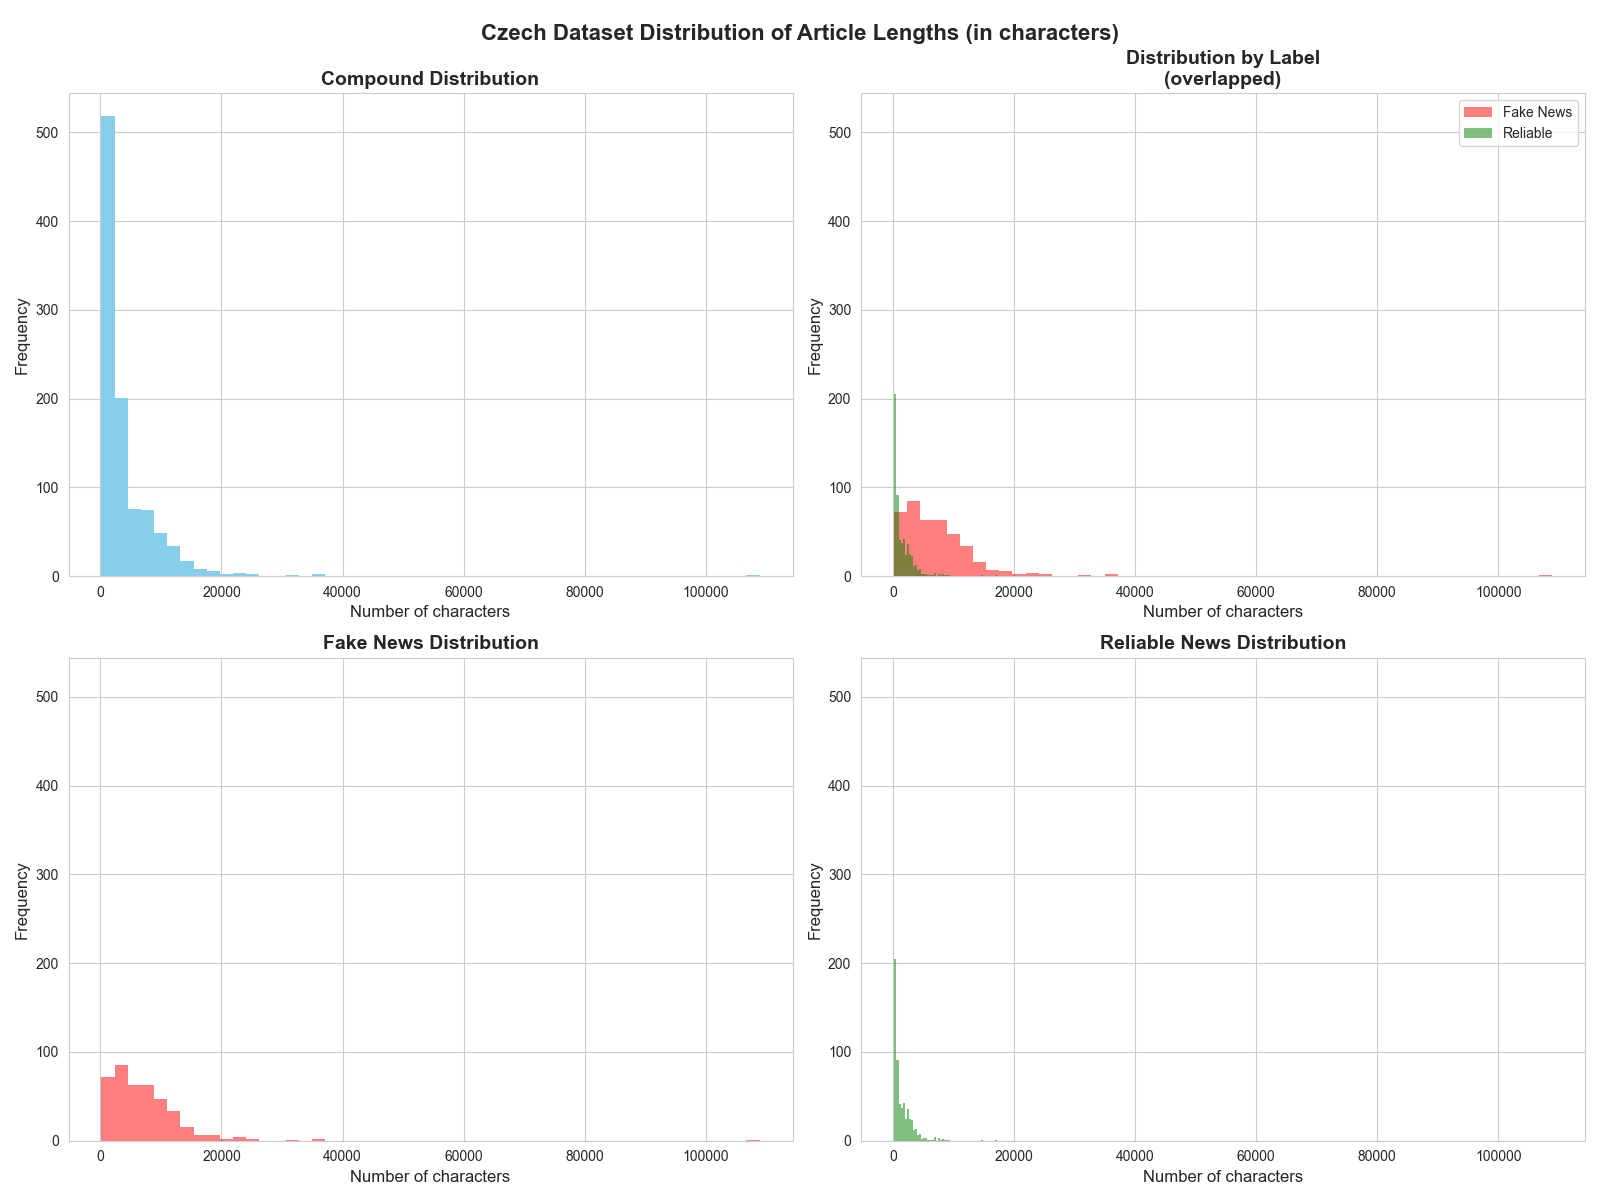
\includegraphics[width=\linewidth]{text/chapters/3-datasets/assets/cz_dataset/article_lengths_distribution.png}
%     \caption{Czech dataset distribution of article lengths}
%     \label{fig:cz_dataset_article_lengths_distr}
% \end{figure}


% \subsection{Tokenization Analysis}

% \begin{figure}[!htbp]
%     \centering
%     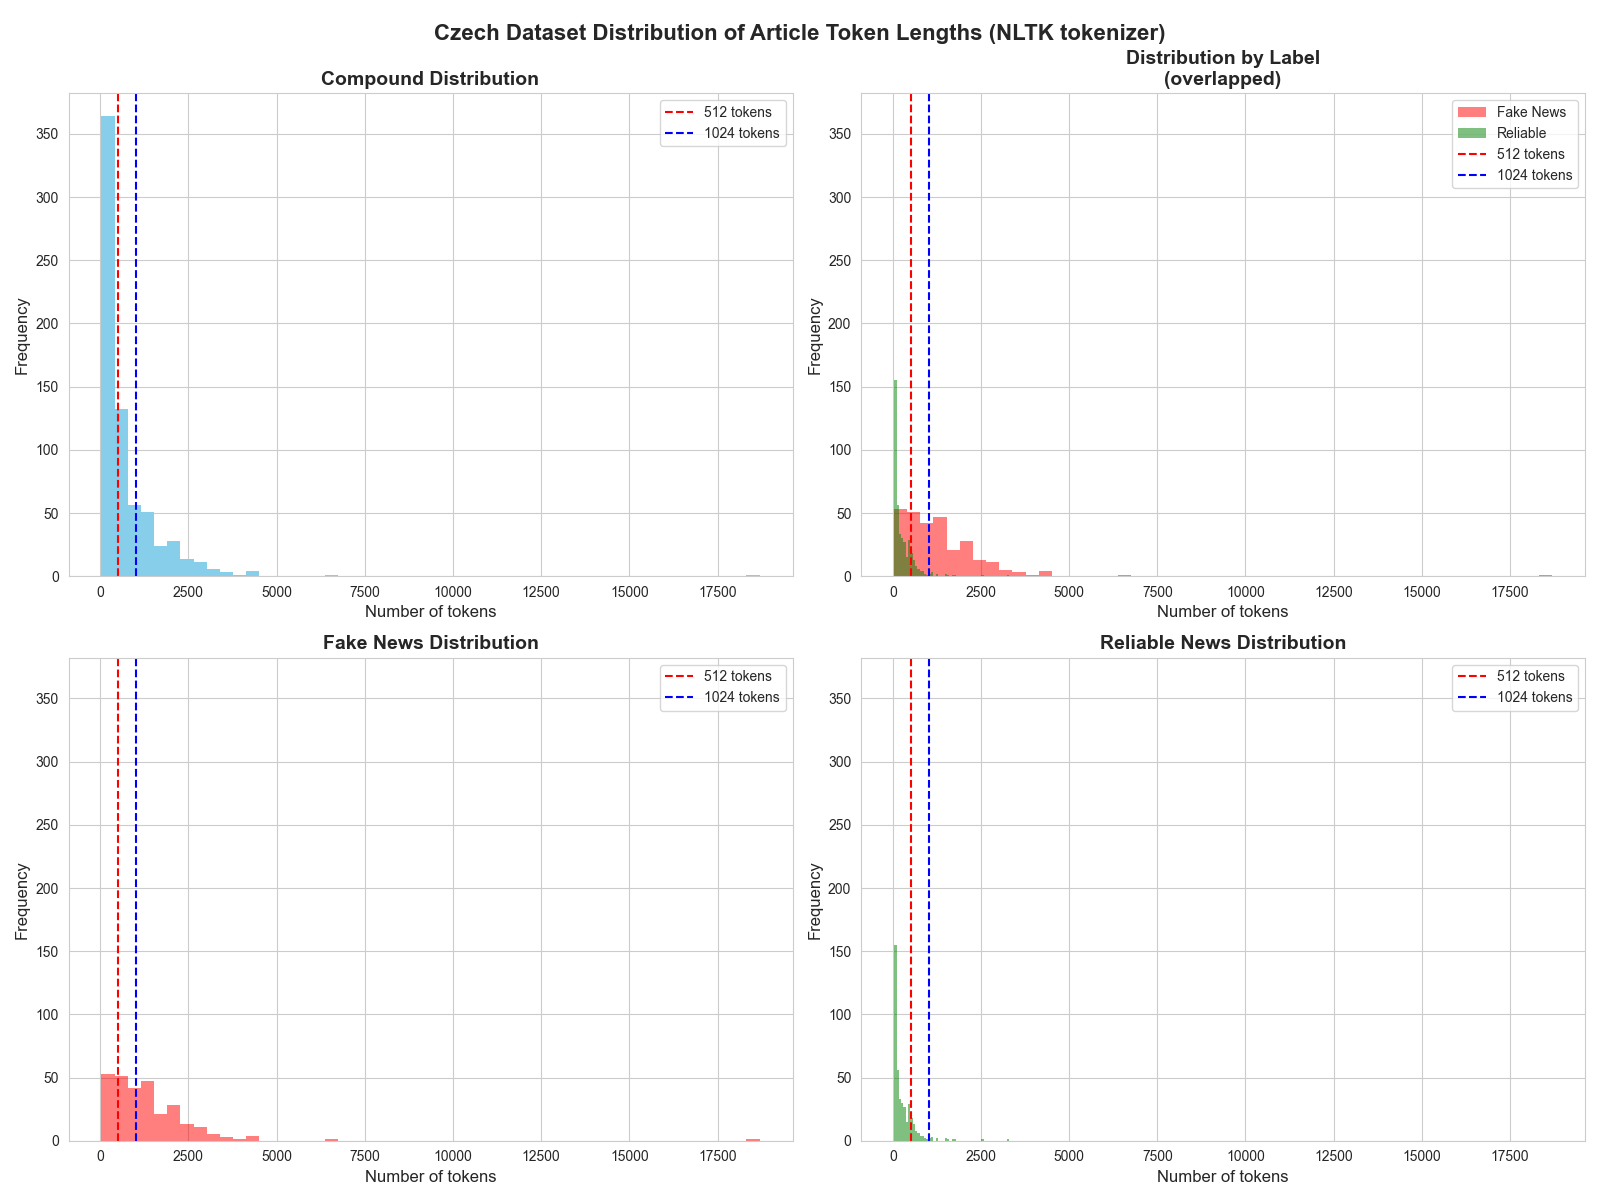
\includegraphics[width=\linewidth]{text/chapters/3-datasets/assets/cz_dataset/nltk_token_length_distribution.png}
%     \caption{Czech dataset distribution of token lengths (NLTK tokenizer)}
%     \label{fig:cz_dataset_nltk_token_length_distr}
% \end{figure}


% \begin{figure}[!htbp]
%     \centering
%     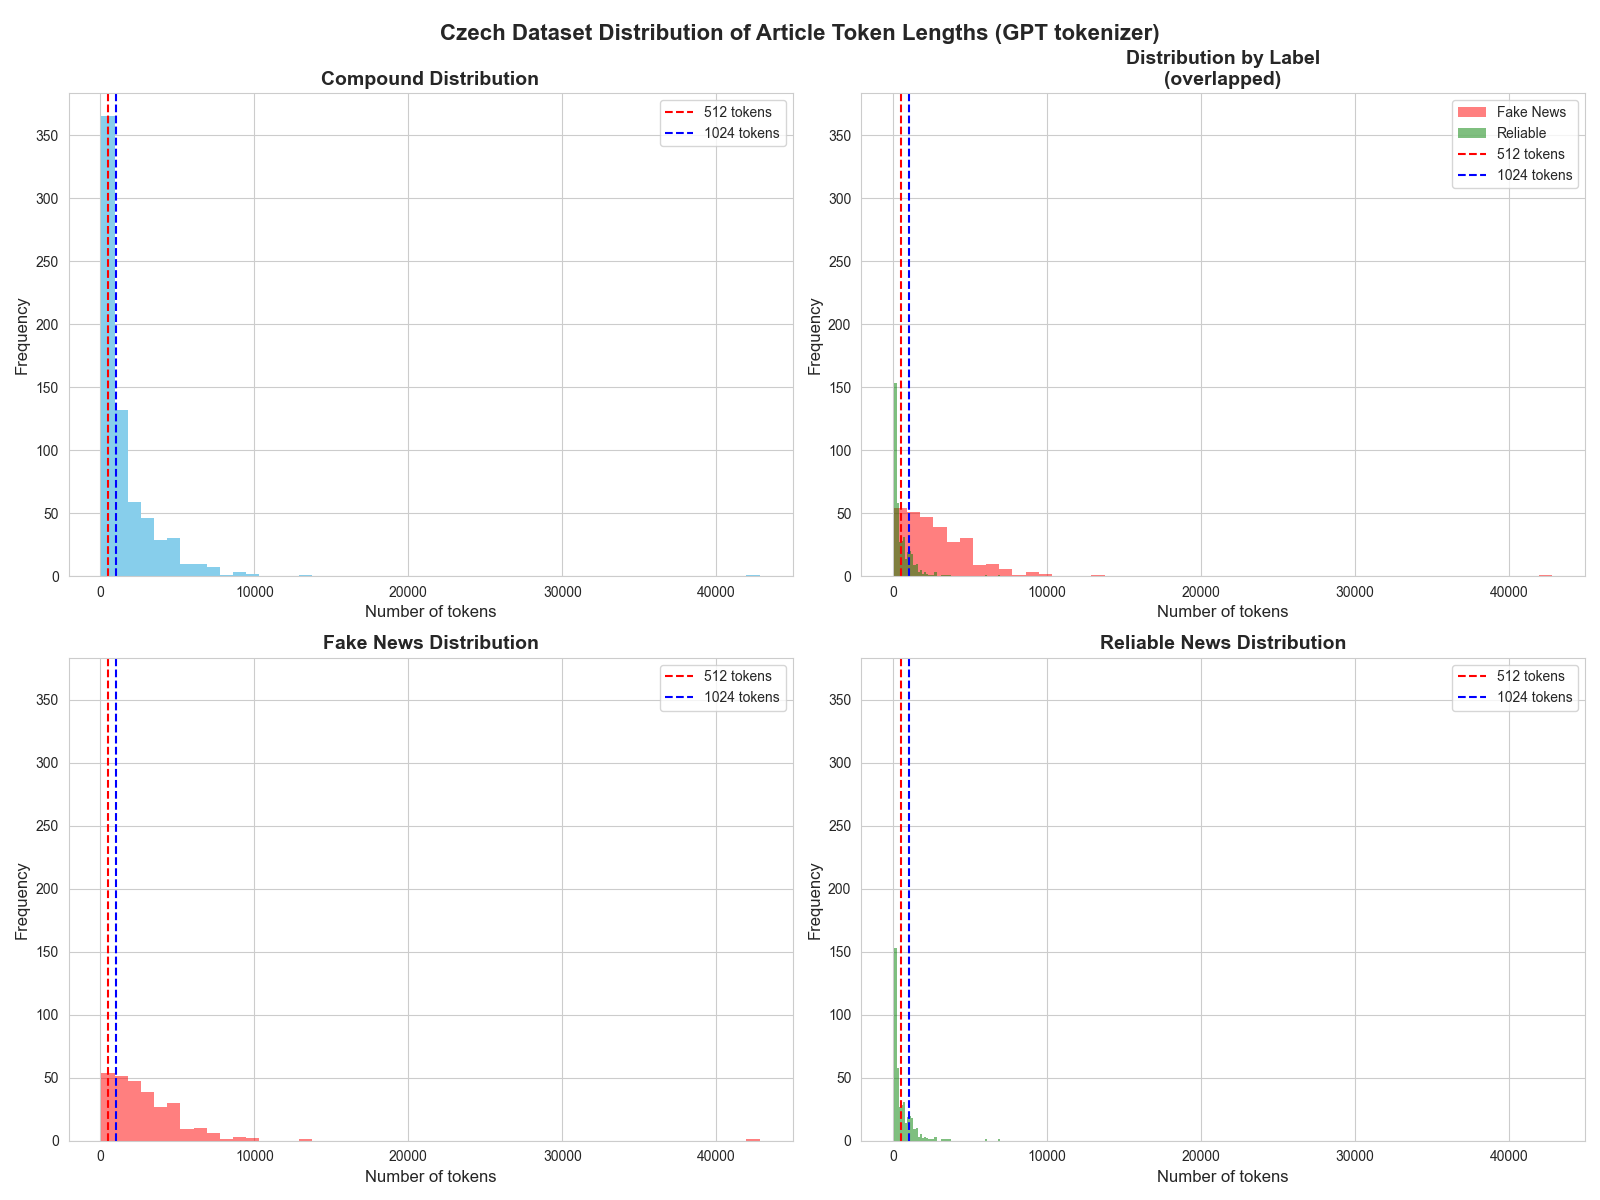
\includegraphics[width=\linewidth]{text/chapters/3-datasets/assets/cz_dataset/gpt_token_length_distribution.png}
%     \caption{Czech dataset distribution of token lengths (GPT-1 tokenizer)}
%     \label{fig:cz_dataset_gpt_token_length_distr}
% \end{figure} % include `appendix.tex' from `text/' subdirectory

%%%%%%%%%%%%%%%%%%%
% APPENDIX INCLUDE END
%%%%%%%%%%%%%%%%%%%

\backmatter % do not remove this command

\printbibliography % print out the BibLaTeX-generated bibliography list

% !!!!!!!!!!!!!!!!!!!!!!!!! include in final version !!!!!!!!!!!!!!!!!!!!!!!!!
\chapter{Contents of attached medium}


The attached medium contains the source code for the implemented experiments, as well as visualization scripts, analytical notebooks, and execution notebooks for running and training the experimental models.


\bigskip


\dirtree{%
.1 materials.
.2 BP Flajžík Jan\dotfill{}original thesis \cite{flajzik_classification_2024} text and sources.
.2 {etc...} \dotfill{}other materials.
.1 workspace.
.2 mlruns\dotfill{}logs used in the MLflow.
.2 notebooks\dotfill{}training and visualizations.
.2 sources\dotfill{}reusable python modules.
.3 experiments\dotfill{}package with experiment runs logic.
.3 local\_datasets\dotfill{}datasets analysis and preprocessing.
.3 models\dotfill{}machine learning models logic.
.3 {\_\_init\_\_.py}.
.3 {utils.py}.
.2 tests.
.1 {README.md}.
.1 {.gitignore}.
.1 requirements.txt \dotfill{} packages to install.
} % include `medium.tex' from `text/' subdirectory

\end{document}
